\chapter{Algorithm}
\label{ch:algorithm}

The original goal of the preference reward algorithm was to transfer learned behavior from one RL agent to another. It is, however, designed to only rely on an abstract interface of the source of knowledge, the teacher. A teacher, as described in definition \ref{def:teacher}, if given a state, proposes an action together with a confidence about the quality of this action.
\begin{definition}
    \label{def:teacher}
     Let $(S, A, P, R, \rho_0, \gamma)$ be a MDP. Then a function $$T: S \rightarrow A\times[0,1]$$ is called a \emph{teacher} for this MDP. A teacher proposes an action for each state and gives a confidence about the quality of this action.
\end{definition}
In practice, a teacher does not necessarily has to be a RL agent, but can also be a trajectory planner or other means of solving the task at hand. See section \ref{sec:teachers} about different kinds of teachers. The following section \ref{sec:preference-reward} outlines the preference reward algorithm.

\section{Preference Reward}
\label{sec:preference-reward}

The preference reward algorithm uses reward shaping to assist the exploration of a RL agent in training. It can therefore be used with any RL algorithm. The reward is changed based on the actions that a teacher suggests for the current state. This action is considered the preferred action. See section \ref{sec:teachers} for details about teachers.

Three different rewards are used for an MDP and a teacher $T$, the \emph{environment reward}, \emph{teacher reward} and \emph{preference reward}. See definition \ref{def:preference-reward}. First, the reward from the MDP is called \emph{environment reward} $r_{env}$. For a state $s$ and an action $a$ proposed by the agent, the teacher gives an action $\hat{a}$ and a confidence $c$. The confidence is used by the teacher to rate the quality of its action $\hat{a}$. The mean square error, of $a$ and $\hat{a}$ is called the \emph{action error}. The action error, multiplied with the negated confidence forms the \emph{teacher reward} $r_{teacher}$. The teacher reward may be seen as a penalty for the agent if the proposed actions are not in line with the teachers actions. The confidence makes sure that the penalty is lower if the teacher is not confident about the quality of its action. Lastly, the weighted sum of the environment and teacher reward is called \emph{preference reward} $r_{pr}$. The importance of the teacher reward is determined by a parameter $\alpha \in [0,1]$.
\begin{definition}
    \label{def:preference-reward}
    Let $(S, A, P, R, \rho_0, \gamma)$ be a MDP, $T$ a teacher, $(s, a, s')$ a state, action, next state triplet, and $\alpha \in [0,1]$. Then:
    \begin{enumerate}[(1)]
        \item\label{enm:pr:external-reward} $r_{env} = R(s, a, s')$ is called \emph{environment reward}.
        \item\label{enm:pr:internal-reward} Let $T(s) = (\hat{a}, c)$. Then $r_{teacher} = -c * \frac{1}{dim(A)} \sum_i (a_i - \hat{a}_i)^2$ is called \emph{teacher reward}.
        \item\label{enm:pr:preference-reward} $r_{pr} = \alpha * r_{teacher} + (1-\alpha) * r_{env}$ is called \emph{preference reward}.
    \end{enumerate}
\end{definition}

Algorithm \ref{alg:preference-reward} outlines the steps to calculate the preference reward. First, the teacher is used to obtain the preferred action $\hat{a}$ and the confidence $c$. Together with the action $a$ from the agent, the teacher reward is calculated. Lastly, the preference reward is calculated from the environment reward and the teacher reward.
\begin{algorithm}[btp]
    \caption{Preference Reward}
    \label{alg:preference-reward}

    \DontPrintSemicolon
    \SetFuncSty{textsc}
    
    \KwIn{action $a \in \mathbb{R}^n$, state $s$, reward $r_{env}$, teacher $T$, $\alpha \in [0,1]$}
    \KwData{$\hat{a} \in \mathbb{R}^n$, $c \in \mathbb{R}$, $r_{teacher} \in \mathbb{R}$}
    \KwOut{preference reward $r_{pr} \in \mathbb{R}$}

    \SetKwFunction{predict}{predict}
    \SetKwFunction{random}{selectRandomElement}
    \SetKwFunction{std}{standardDeviation}
    \SetKwFunction{exp}{exp}
    
    \BlankLine
    $\hat{a}, c \leftarrow T(s, a)$\;
    $r_{teacher}\leftarrow -c * \frac{1}{n} \sum_{i=0}^n(a_i-\hat{a}_i)^2$\;
    $r_{pr}\leftarrow \alpha * r_{teacher} + (1-\alpha) * r_{env}$\;
    return $r_{pr}$\;
\end{algorithm}

\subsection{Adaptive Alpha}
\label{sec:adaptive-alpha}

The parameter $\alpha$ that determines the importance of the preference reward does not necessarily need to be a fixed value. It is possible to change the value of $\alpha$ based on different factors. In fact, it turned out to increase the success rate of the agent, to reduce the $\alpha$ value as the training progressed. See the experiment results in section \ref{sec:experiments:results}. We explored two methods for adapting $\alpha$ during training: one based on the number of training steps completed, and another based on the rewards our agent was receiving in its environment

For an adaptive $\alpha$ based on training steps, the $\alpha$ with a value of one and is linearly reduced to zero at the final training step. The adaptive $\alpha$ based on the environment reward assumes that the agent is getting better if the environment reward increases and therefore does not need as much guidance from the teacher. To make the $\alpha$ value more stable, we used an exponential moving average of the environment reward to calculate it.

Other options to adapt $\alpha$ are possible, but we leave them for future work.

\subsection{High Dimensional Observations}
\label{sec:algo-high-dim-observations}

In this work, the preference reward algorithm was used to assist the training of a SAC agent using high dimensional image observations, assuming that during training, the full state of the environment is available. Figure \ref{fig:algorithm} shows the training setup. The SAC agent only relies on a frame stack as observations, the state is only needed for the teacher during training. Optionally, the gripper position can be added to the observation, to simplify the task. The gripper position could be obtained from a real world robot and does therefore not break the goal to train under realistic assumptions.

The idea behind this setup is to utilize more information during training than during evaluation. In a real world application, this would result in using more sensors during training to measure the state of the environment and use it for the teacher. But during evaluation, the trained agent only relies on simple sensor data, such as images and the gripper position.

\begin{figure}[btp]
    \centering
    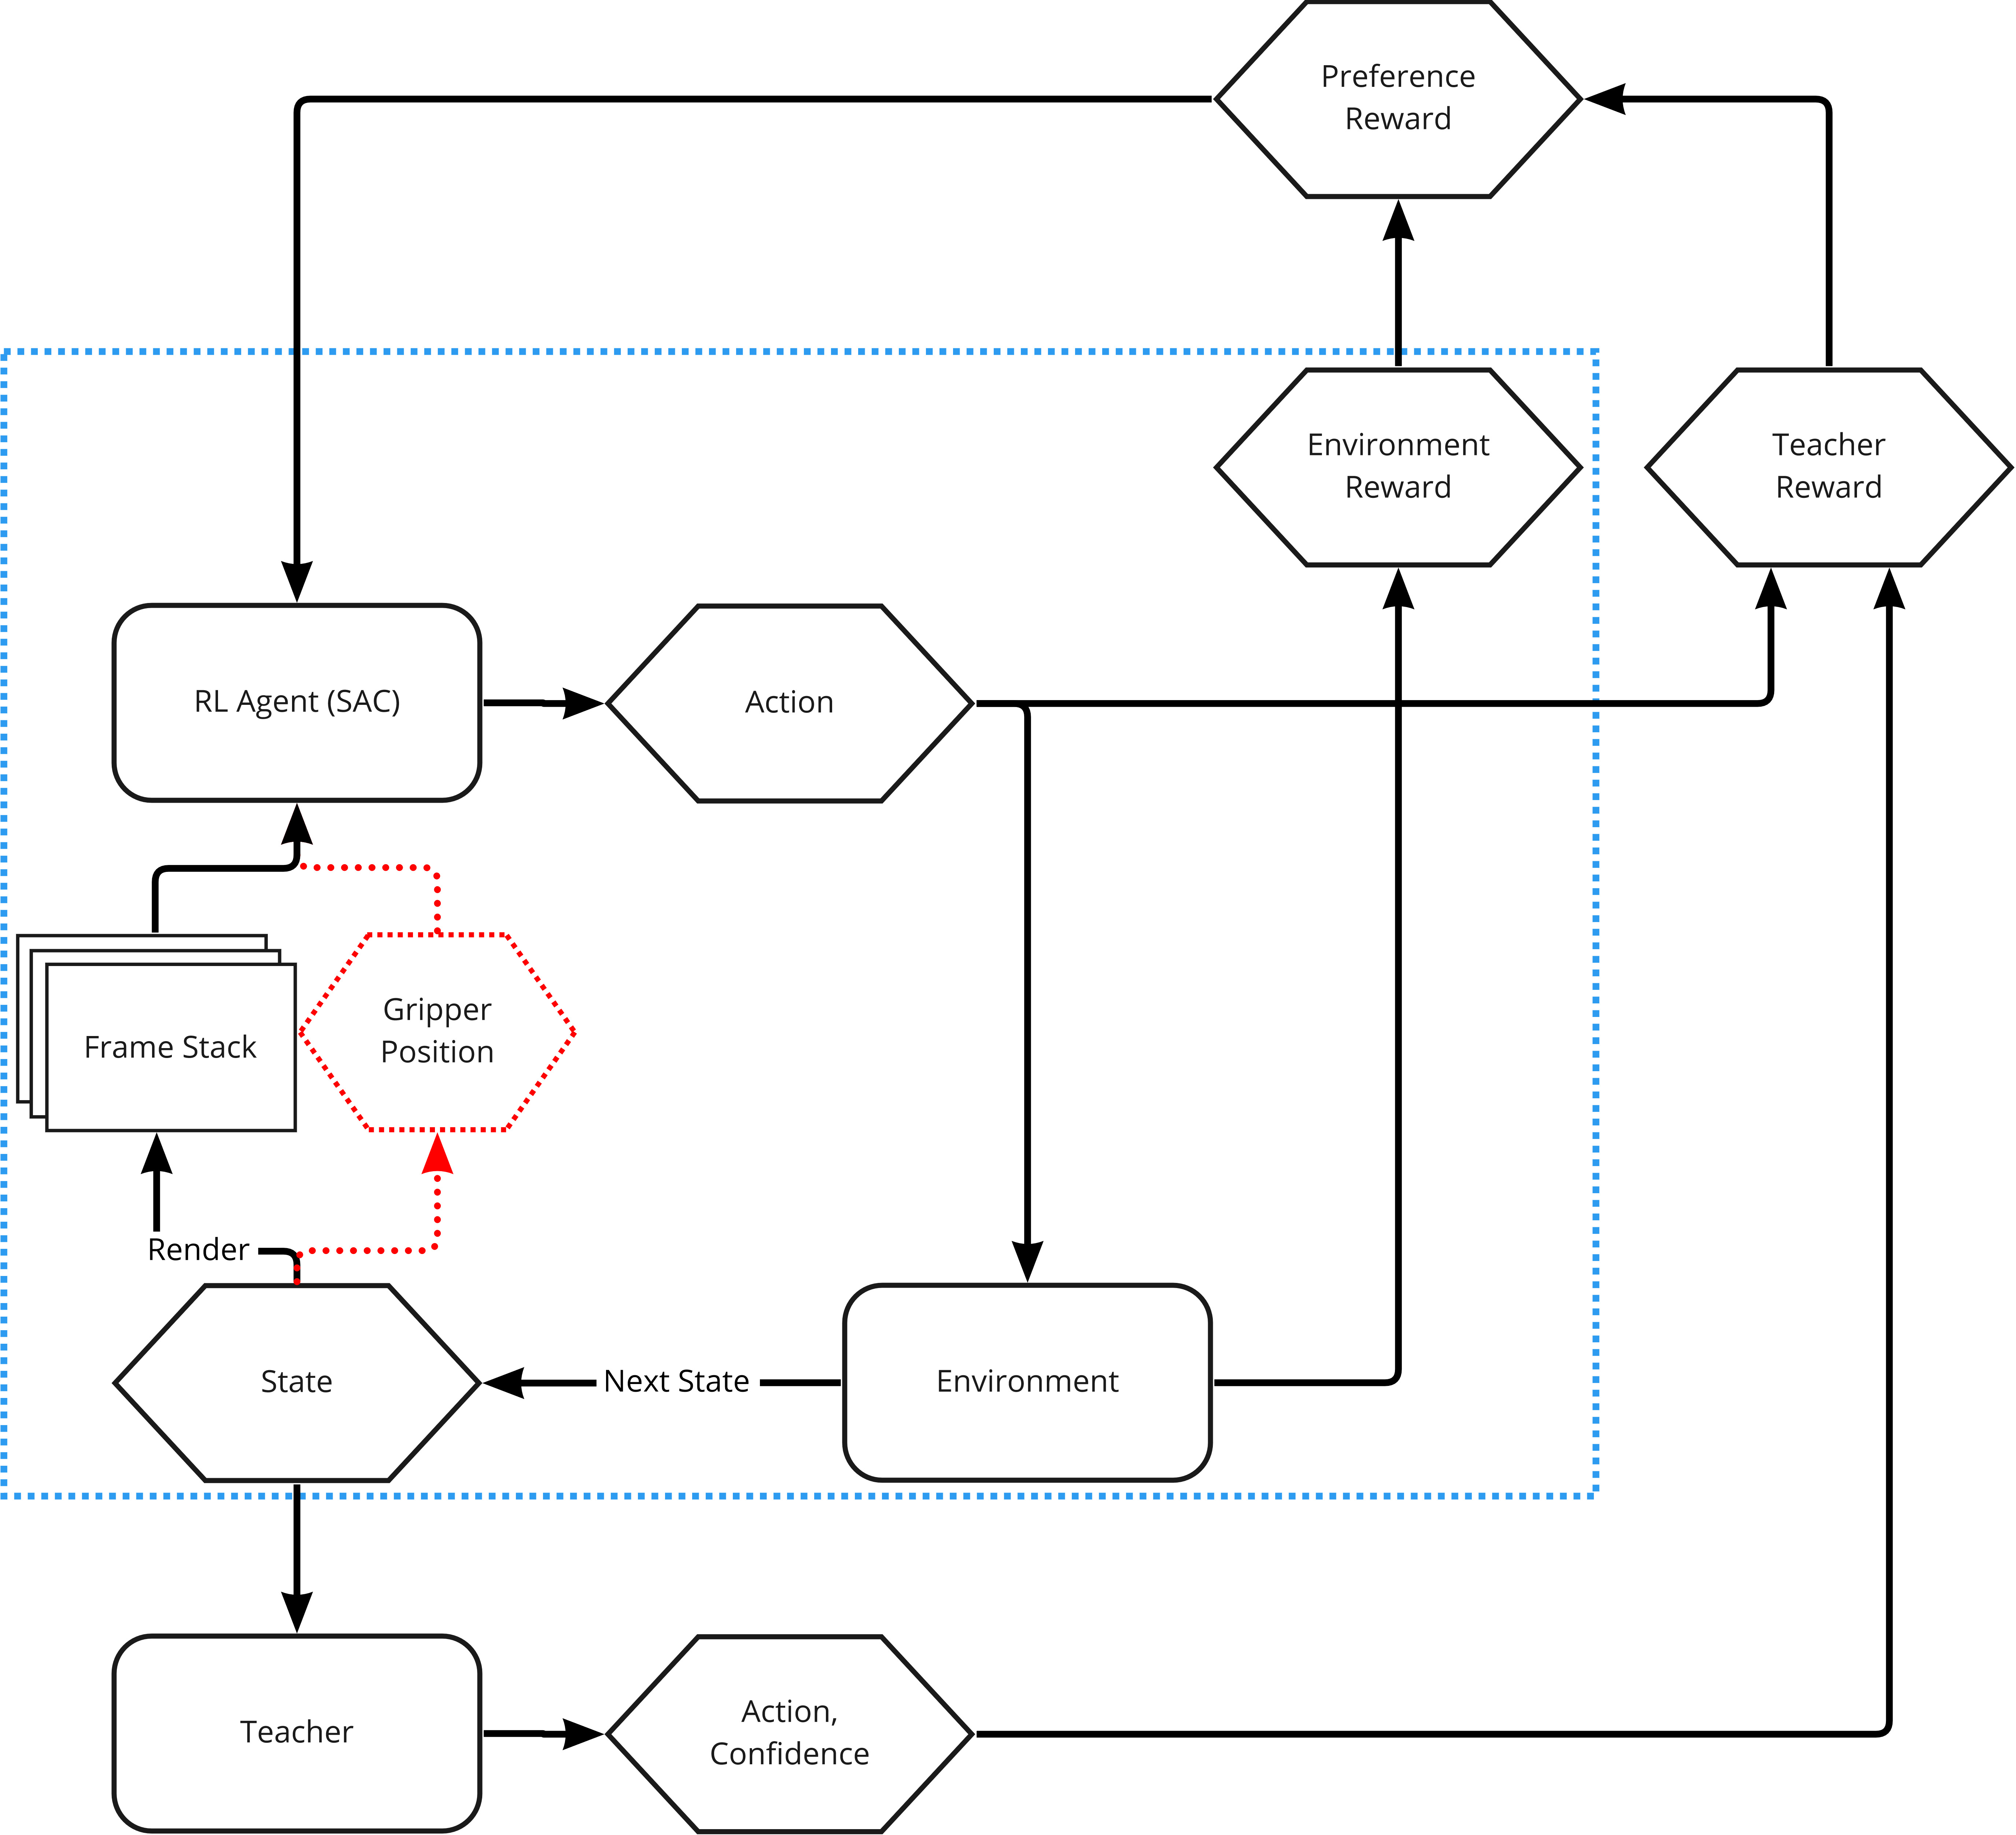
\includegraphics[width=\textwidth]{images/algorithm.jpg}
    \caption[Overview of the preference reward algorithm]{Overview of the preference reward algorithm to train an agent on high dimensional image observations. Optionally, the gripper position of a robot can be added to the observation. The elements marked in blue are present in regular SAC.}
    \label{fig:algorithm}
\end{figure}

\subsection{Teachers}
\label{sec:teachers}

As stated in definition \ref{def:teacher}, a teacher is a function that proposes an action for each state and provides a confidence about the quality of this action. For the training setup as described in section \ref{sec:algo-high-dim-observations}, the teacher may use a RL agent trained on the full state of the environment to obtain the preferred action. To obtain the confidence, algorithm \ref{alg:ensemble-teacher} uses an ensemble of multiple teachers. First, the element wise standard deviation is calculated. Then the exponential of the negative standard deviation is used as confidence, to ensure a range of $[0,1]$. From the actions proposed by the agents of the ensemble, one is drawn at random as the preferred action. Note that in this case, the teacher is not a mathematical function, as it is not deterministic. Another way to obtain the confidence with just a single agent is to use dropout as Bayesian approximation, as described in \cite{galDropoutBayesianApproximation2016}.

The training setup described in section \ref{sec:algo-high-dim-observations} and figure \ref{fig:algorithm} is not the only setup where a RL agent can be used as a teacher. In a slightly modified version of this setup, where the teacher and the student both receive the same observation, it is still possible to utilize an RL agent as a teacher. While the teacher would not be able to solve the task at hand perfectly, it could be an agent that can solve a simpler sub task and therefore guide the exploration of the agent in training.

However, the teacher does not necessarily has to be an RL agent. Other means to propose an action may be used as teachers as well. They only need to fulfill definition \ref{def:teacher}, that is being able to provide an action and a confidence for each state. One example would be a trajectory planner.

\begin{algorithm}[btp]
    \caption{Ensemble Teacher}
    \label{alg:ensemble-teacher}

    \DontPrintSemicolon
    \SetFuncSty{textsc}
    
    \KwIn{action $a \in \mathbb{R}^n$, state $s$, list of RL agents $L$}
    \KwData{list of actions $A$}
    \KwOut{action $\hat{a} \in \mathbb{R}^n$, confidence $c \in [0,1]$}

    \SetKwFunction{append}{append}
    \SetKwFunction{predict}{getAction}
    \SetKwFunction{random}{selectRandomElement}
    \SetKwFunction{std}{standardDeviation}
    \SetKwFunction{exp}{exp}
    
    \BlankLine
    \tcp{L is only provided when initializing the teacher and not each time}
    \ForEach{$agent$ in $L$}
    {$A$.\append(agent.\predict(s))}
    $\hat{a} \leftarrow\random{A}$\;
    $c \leftarrow\exp(-\std(A))$\;
    return $\hat{a}, c$\;
\end{algorithm}

\section{Safety}
\label{sec:safety}

As described in section \ref{sec:preliminaries:rl:cmdp}, a constrained Markov decision process is a MDP extended by a cost function $C(s,a,s')\rightarrow[0,1]$ and a threshold $\delta \in \mathbb{R}_{\geq 0}$. Three different approaches were attempted in this work to extend SAC to CMDPs. The goal with these was not to strictly stay below the threshold $\delta$, but to learn a policy that minimizes the expected cost of an episode. One of the approaches uses reward shaping and the other two a safety critic.

\subsection{Reward Based}
\label{sec:reward-based}

The first, and simplest approach is to penalize the agent by deducting the cost of a state, action, next state triplet $(s, a, s')$ from the reward:
\begin{equation}
    \label{eq:reward-based-cost}
    R_{cost}(s,a,s') = \lambda_r R(s,a,s') - \lambda_c C(s,a,s')
\end{equation}
The parameters $\lambda_r, \lambda_c \geq 0$ symbolize the importance of the reward and the cost. With this approach, the new reward function $R_{cost}$ is not guaranteed to be in the interval $[0,1]$.

\subsection{Safety Critic}
\label{sec:safety-critic}

The cost is defined in the same way as the reward, the only difference is that the goal is to minimize the cost while the reward should be maximized. It is therefore possible to formulate the value functions and bellman equations $V^\pi(s)$ and $Q^\pi(s,a)$ just like in section \ref{sec:preliminaries:rl:valueFunctions}. In the following, an index $R$ or $C$ is added to the functions to indicate whether they are the reward or safety function. The parameter vectors for the Q-function neural networks are indexed in the same way as $\phi^C_i$ and $\phi^R_i$, where $i$ is the index for the double-Q trick. 

The functions for the optimal policy $V_C^*(s)$ and $Q_C^*(s,a)$ can not be formulated just like that, because the goal is not to minimize the cost but to maximize the reward while maintaining a low cost. It is therefore not clearly defined what the optimal policy is. The same is true for the reward function regarding the optimal policy $V_R^*(s)$ and $Q_R^*(s,a)$. This is, however, not a problem, since the optimal policy functions are not needed for SAC.

Together with the entropy, this results in the following cost Bellman equation similar to equation \ref{eq:sac-bellman-q-3}:
\begin{equation}
    Q_C^\pi(s,a) = \underset{\begin{subarray}{c}
        s'\sim P(\cdot|s,a)\\
        a'\sim\pi
    \end{subarray}}{\mathbb{E}}\Big[C(s,a,s') + \gamma\Big(Q_C^\pi(s',a') - \alpha \log\pi(a'|s')\Big)\Big]
    \label{eq:sac-cost-bellman}
\end{equation}

During training, the replay buffer also stores the cost of a transition. A sample from it is therefore a sextuple $(s,a,r,c,s',d)$, where c denotes $C(s,a,s')$. With this, similar to equation \ref{eq:q-approx}, the safety-Q can be approximated:
\begin{equation}
    Q_C^\pi(s,a) \approx c+\gamma(Q_C^\pi(s',a')-\alpha \log~ \pi(a'|s')),~ a'\sim\pi(\cdot|s')
    \label{eq:safety-q-approx}
\end{equation}
Again, this is used to create the target function:
\begin{equation}
    y_C(c,s',d) = c+\gamma(1-d)\Big(\underset{j=1,2}{\max}Q_{\overline{\phi}^C_i}(s',a')-\alpha \log~ \pi_\theta(a'|s')\Big),~ a'\sim\pi_\theta(\cdot|s')
    \label{eq:safety-q-target}
\end{equation}
Just like for the reward critic, older versions of the two Q-functions are used to calculate the target. This stabilizes the training. They are denoted with ${\overline{\phi}^C_i}$. Note that in contrast to equation \ref{eq:q-target} the maximum of the two Q-functions is used.
Just like the reward critic, the safety critic can be trained with:
\begin{equation}
    J_{Q_C}(\phi)_i = \underset{(s,a,r,c,s',d)\sim D}{\mathbb{E}}\Big[\Big(Q_{\phi^C_i}(s,a)-y_C(c,s',d)\Big)^2\Big]
\end{equation}

In this work, two different ways to use the safety critic were evaluated. One is to use the safety critic during the training of the policy. The other approach only uses the safety critic in the evaluation.

\subsubsection{Safety Training}
\label{sec:safety-training}

The first approach using the safety critic changes the training objective of the actor. Instead of training an actor that is proportional to the exponential of the Q-function, it should now be proportional to the difference between the reward and safety critic:
\begin{equation}
    \pi(a| s) \propto \exp(Q_R(s, a) - Q_C(s,a))
\end{equation}
This also changes the goal to minimize the Kullback-Leibler divergence between the actor and the exponential difference between the two critics:
\begin{align}
    & \underset{s\sim D}{\mathbb{E}}\Bigg[D_{KL}\Bigg(\pi_\theta(\cdot|s)\Bigg|\Bigg|\frac{\exp\big(\frac{1}{\alpha}(Q_{\phi^R}(s,\cdot)-Q_{\phi^C}(s,\cdot))\big)}{Z_\phi(s)}\Bigg)\Bigg]\\
    &= \underset{s\sim D}{\mathbb{E}}\Bigg[\sum_{a\in A} \pi_\theta(a|s) \log\Bigg(\frac{\pi_\theta(a|s)Z_\phi(s)}{\exp\big(\frac{1}{\alpha}(Q_\phi^R(s,a)-Q_{\phi^C}(s,\cdot))\big)}\Bigg)\Bigg]\\
    &= \underset{\begin{subarray}{c}
        s\sim D\\
        a\sim \pi_\theta(\cdot|s)
    \end{subarray}}{\mathbb{E}}\Big[\log\pi_\theta(a|s)+\log Z_\phi(s)-\frac{1}{\alpha}(Q_{\phi^R}(s,a)-Q_{\phi^C}(s,\cdot))\Big]\\
    &= \underset{\begin{subarray}{c}
        s\sim D\\
        a\sim \pi_\theta(\cdot|s)
    \end{subarray}}{\mathbb{E}}\Big[\alpha\log\pi_\theta(a|s)+\alpha\log Z_\phi(s)-Q_{\phi^R}(s,a)+Q_{\phi^C}(s,\cdot)\Big]
\end{align}
Just like it is done for regular SAC in equation \ref{eq:pi-kl-3}, the term $Z_\phi(s)$ can be omitted and the equation is multiplied by $\alpha$ to get the new training objective:
\begin{equation}
    J_\pi(\theta) = \underset{\begin{subarray}{c}
        s\sim D\\
        a\sim \pi_\theta(\cdot|s)
    \end{subarray}}{\mathbb{E}}\Big[\alpha\log\pi_\theta(a|s)-Q_{\phi^R}(s,a)+Q_{\phi^C}(s,\cdot)\Big]
    \label{eq:pi-cost-objective-no-reparam}
\end{equation}
Again similar to regular SAC, the reparametrization trick from equation \ref{eq:reparam-trick} has to be used. Additionally the double Q-trick is added for both critics, resulting in the following objective:
\begin{equation}
    J_\pi(\theta) = \underset{\begin{subarray}{c}
        s\sim D\\
        \xi\sim \mathcal{N}(0, I)
    \end{subarray}}{\mathbb{E}}\Big[\alpha\log\pi_\theta(f_\theta(s, \xi)|s)-\underset{i=1,2}{\min}Q_{\phi_i^R}(s,f_\theta(s, \xi))+\underset{i=1,2}{\max}Q_{\phi_i^C}(s,f_\theta(s, \xi))\Big]
    \label{eq:actor-loss-cost}
\end{equation}
Note that in order to use the more pessimistic of the two safety critics, the maximum of the two has to be used. This leads to some changes in the SAC algorithm, as described in algorithm \ref{alg:sac}. In addition to the updates to the reward critic, now at ever step also the safety critic is updated. To do so, also the safety critic targets need to be updated. Finally, the actor is trained with the new objective from equation \ref{eq:actor-loss-cost}. The new algorithm is described in detail in algorithm \ref{alg:sac-safety-critic}

\begin{algorithm}[btp]
    \caption{Safety SAC}
    \label{alg:sac-safety-critic}

    \DontPrintSemicolon
    \SetFuncSty{textsc}
    
    \KwIn{entropy coefficient $\alpha$, environment $e$, initial parameters $\theta, \phi^R_1, \phi^R_2, \phi^C_1, \phi^C_2$, learning rates $\eta_\pi$, $\eta_Q$, target update rate $\rho$}
    \KwData{replay buffer $D$}
    \KwOut{$\theta, \phi^R_1, \phi^R_2,\phi^C_1,\phi^C_2$}

    \SetKwFunction{append}{append}
    \SetKwFunction{initialstate}{initialState}
    \SetKwFunction{step}{step}
    \SetKwFunction{reset}{reset}
    
    \BlankLine
    \tcp{Initialize target networks}
    $\overline{\phi}^R_1 \gets \phi^R_1$, $\overline{\phi}^R_2 \gets \phi^R_2$\;
    $\overline{\phi}^C_1 \gets \phi^C_1$, $\overline{\phi}^C_2 \gets \phi^C_2$\;
    $s\gets e.\initialstate()$\;
    
    \For{each iteration}{
        \tcp{Interact with the environment}
        $a\sim \pi_\theta(\cdot|s)$\;
        $r, c, s', d\gets e.\step(a)$\;
        $D.\append((s,a,r,c,s',d))$\;
        \If{$d = done$}{
            $e.\reset()$\;
            $s\gets e.\initialstate()$\;
        }
        Sample a batch $B$ of transitions from $D$\;
        \tcp{Compute Q-function targets}
        \ForEach{$(s,a,r,c,s',d)\in B$}{
            $y_R(r,s',d) \gets r+\gamma(1-d)\Big(\underset{j=1,2}{\min}Q_{\overline{\phi}^R_i}(s',a')-\alpha \log~ \pi_\theta(a'|s')\Big),~ a'\sim\pi_\theta(\cdot|s')$\;
            $y_C(c,s',d) \gets c+\gamma(1-d)\Big(\underset{j=1,2}{\max}Q_{\overline{\phi}^C_i}(s',a')-\alpha \log~ \pi_\theta(a'|s')\Big),~ a'\sim\pi_\theta(\cdot|s')$\;
        }
        \tcp{Update Q-functions and policy by one step of gradient descent}
        \For{$i=1,2$}{
            $\phi^R_i\gets \phi^R_i - \eta_Q\nabla_{\phi^R_i}\frac{1}{|B|} \sum_{(s,a,r,c,s',d)\in B}\Big[\Big(Q_{\phi^R_i}(s,a)-y_R(r,s',d)^2\Big)\Big]$\;
            $\phi^C_i\gets \phi^C_i - \eta_Q\nabla_{\phi^C_i}\frac{1}{|B|} \sum_{(s,a,r,c,s',d)\in B}\Big[\Big(Q_{\phi^C_i}(s,a)-y_C(r,s',d)^2\Big)\Big]$\;
        }
        \For{$i = 1,2,\dots,|B|$}{
            $\xi_i\gets \mathcal{N}(0,I)$\;
        }
        $\theta\gets \theta - \eta_\pi\nabla_\theta\frac{1}{|B|} \sum_{s\in B}\Big[\alpha\log\pi_\theta(f_\theta(s, \xi)|s)-\underset{i=1,2}{\min}Q_{\phi_i^R}(s,f_\theta(s, \xi))+\underset{i=1,2}{\max}Q_{\phi_i^C}(s,f_\theta(s, \xi))\Big]$\;
        \tcp{Update target networks}
        \For{$i=1,2$}{
            $\overline{\phi}^R_i\gets \rho\overline{\phi}^R_i + (1-\rho)\phi^R_i$\;
            $\overline{\phi}^C_i\gets \rho\overline{\phi}^C_i + (1-\rho)\phi^C_i$\;
        }
        return $\theta, \phi^R_1, \phi^R_2,\phi^C_1,\phi^C_2$\;
    }
\end{algorithm}

\subsubsection{Safety Evaluation}
\label{sec:safety-eval}

The second approach uses the safety critic only during the evaluation. The safety critic is trained alongside the reward critic, but only the reward critic is used to train the actor. The agent does not consider the cost of the actions during training. It is, therefore, expected to produce high cost actions during training. This makes this approach only viable for tasks where, during training, neither the actor nor the environment is likely to break due to high cost actions.

When the agent is evaluated, or used in practice, the trained safety critic comes into play. SAC trains a stochastic actor. However, a deterministic version of the actor is usually used for the evaluation. This can be achieved by not applying any randomization in the reparametrization trick and directly returning $\mu_\theta(s)$ as the action. See equation \ref{eq:reparam-trick} for reference. The safety evaluation algorithm relies on the stochastic nature of a SAC actor. Therefore, the stochastic version of the actor is used during evaluation when using the safety evaluation algorithm.

The safety evaluation algorithm is described in algorithm \ref{alg:safety-eval}. Its goal is to select an action for a state that has a low cost. The stochastic actor makes it possible to sample $n$ different actions for a state. For each action, the expected cost is calculated with the safety critic. First, it is checked if any of the actions has an expected cost of less than a threshold $\delta$. If this is not the case, the action with the lowest expected cost is returned. If some actions suffice the cost threshold $\delta$, the expected reward for each of them is calculated using the reward critic. The action with the highest expected reward is returned.

\begin{algorithm}[btp]
    \caption{Safety Evaluation}
    \label{alg:safety-eval}

    \DontPrintSemicolon
    \SetFuncSty{textsc}
    
    \KwIn{state $s$, actor $A$, reward critic $Q_R$, safety critic $Q_C$, number of samples $n$, safety threshold $\delta$}
    \KwData{list of action, cost tuples $L$}
    \KwOut{action $a$}

    \SetKwFunction{append}{append}
    \SetKwFunction{predict}{sampleAction}

    \SetKwFor{For}{do}{times}{endfor}
    
    \BlankLine
    \For{$n$}{
    $a\gets A.\predict(s)$\;
    $c\gets Q_C(s,a)$\;
    $L.\append((a,c))$\;
    }
    \eIf{$\exists (a,c)\in L: c < \delta$}{
        $L\gets \{(a,c)\in L| c < \delta\}$\;
        $(a,c)\gets \underset{(a,c)\in L}{\arg\max}~Q_R(s,a)$\;
        return $a$\;
    }{
        $(a,c)\gets \underset{(a,c)\in L}{\arg\min}~c$\;
        return $a$\;
    }
\end{algorithm}

\section{Implementation Details}
\label{sec:impl-details}

Some aspects of the preference reward algorithm were slightly altered in the implementation when compared to section \ref{sec:preference-reward}. In definition \ref{def:preference-reward}\ref{enm:pr:internal-reward} the teacher reward $r_{teacher}$ is defined as the mean square error between the action of the student and the teacher multiplied by the confidence. The environments used in the evaluation of this work all have an action space of $[-1,1]^4$. This leads to $r_{teacher}$ being in range $[0,4]$. To scale $r_{teacher}$ to the same range as the environment reward $r_{env}$, it is divided by the maximum mean square error possible for the action space, in this case four.

As stated above, the action space has four dimensions. The first three dimension are for the movement in the three dimensional space. The last dimension is used to control the opening of the gripper. See section \ref{sec:experiments:env} for a description of the environments used. The three environments used in this work all ignore the value given to control the opening of the gripper. The fourth dimension is only present to make the environments compatible with others that have the robot pick up the object. To account for the unused fourth dimension, the mean square error in the teacher reward is only calculated over the first three dimensions.

When training on high dimensional image observations, the observations are fed through a CNN encoder, to map them into a smaller latent space. This latent space is then given to the actor and critic networks. The CNN is only trained using the reward critic. The actor and the safety critic use the same CNN as the reward critic for the forward pass, but it is decoupled for the backpropagation.

The implementation can be found under \url{https://github.com/f-krone/SafeTransferLearningInChangingEnvironments}.